\section{Finite Element Methods}
\thispagestyle{plain}

Finite element methods (FEM) are a class of methods for solving PDEs. Advantages include
\begin{itemize}
    \item can work with flexible geometries
    \item handle geometrically intricate boundary conditions
    \item spatially adapt the resolution
\end{itemize}

Generally, numerical schemes need to represent a problem's solution by finitely many numbers,
and then manipulate those numbers as true to the problem as possible. In finite volume
methods we represent the solution as averages on cells which we update based on devised fluxes.
In Smoothed Particle Hydrodynamics, we represent the fluid by a finite set of artificial 
\textit{fluid particles} and update their positions and velocities according to the Lagrangian
form of the fluid equations.

\greenbox{\textbf{Idea of FEMs:} In FEMs the solution domain is structured into finite
elements with nodes on which base functions sit. The partial differential equation (or rather
a weak form\footnote{Weak here means, that the differential equation must not hold strictly locally,
but for instance an integrated residual is to be zero, not the residual everywhere itself.} of it)
turns into equations for the (finitely many) weights of those basis functions.}

\subsection{Finite element methods for linear PDEs}
\subsubsection{The solution is represented by weighted base functions on nodes within finite elements}
The central ideas are
\begin{itemize}
    \item \textcolor{blue1}{Division of space:} The space on which the solution sits is divided into smaller regions called elements (e.g. segments in 1D, rectangles in 2D, cubes, octahedra, ... in 3D).  Every element contains a certain number of points called nodes.
    \item \textcolor{blue1}{Elementwise solution approximation:} We element-wise approximate the solution with a set of linearly independent (not necessarily orthogonal) basis functions evaluated on nodes.
\end{itemize}
On an element we could for instance use a polynomial basis
\begin{equation}
    \text{a line } \phi(x) = a_0 + a_1 x, \quad \text{or a parabula } \phi(x) = a_0 + a_1 x + a_2 x^2
\end{equation}
or Legendre polynomials.
\note{We need the same number of nodes as coefficients so that the values $\phi_i$ on the nodes fully specify our polynomial.}
\greenbox{Better yet, we could use shape function $N$, so that our node values themselves are the coefficients we model.}
So for $n$ node values $\phi_1,\dots,\phi_n$ (called \textit{expansion coefficients}), we can write the solution on the $k$-th element as
\begin{equation}
    \begin{gathered}
        \phi^{(k)}(x) = \phi_1^{(k)} N_1^{(k)}(x) + \phi_2^{(k)} N_2^{(k)}(x) + \dots + \phi_n^{(k)} N_n^{(k)}(x) \\
        \text{shape functions } N_i^{(k)}, \text{ zero outside k-th element}
    \end{gathered}
\end{equation}

\greenbox{All elements use the same base function forms, but for each specific element the sum over its base functions is
only non-zero in the respective element. We can therefore also write the total solution as
\begin{equation}
    \phi(x) = \phi_1 N_1(x) + \phi_2 N_2(x) + \dots + \phi_\mathcal{N} N_\mathcal{N}(x),  \quad \text{in total } \mathcal{N} \text{ nodes}
\end{equation}
}

\note{While we use 1D notation here, we can expand to $\phi(\vec{x}) = \sum_{i=1}^{n} \phi_i N_i(\vec{x})$. Time-dependency can be included as time-dependency of the weights aka expansion coefficients $\phi_i = \phi_i(t)$. But first we will consider constant coefficients, so a stationary (elliptic) problem.}

\bluebox{Based on this the next step is turning the PDE into and algebraic equation for the expansion coefficients $\phi_i$.}

\subsubsubsection{Example 1D linear reconstruction}
A linear 1D example can be seen in figure \ref{fig:1d_linear_reconstruction}.

\begin{figure}[!htb]
    \centering
    \includesvg[width=0.8\textwidth]{figures/1dfem2.svg}
    \caption{1D linear reconstruction}
    \label{fig:1d_linear_reconstruction}
\end{figure}

\subsubsection{From the PDE to an algebraic equation for the expansion coefficients $\phi_1, \dots, \phi_n$}
\yellowbox{For now consider a stationary example (no time dependence of $\phi_j$ in one spatial dimension.)}
\bluebox{In the following we find an algebraic expression (here even a system of linear equations) usually done for the expansion coefficients on one element. Afterwards the equations for all elements have to be assembled (to an overall linear system) in a further step. If the system has $\mathcal{N}$ total nodes, the final linear equation is described by an $\mathcal{N}\times\mathcal{N}$ system. See \cite{lewis2004}.}
\yellowbox{We might sometimes directly find such a system for all expansion coefficients and we will focus on that.}

\subsubsubsection{Inserting the finite element approximation into the PDE yields a residuum}
Consider a linear PDE of the form
\begin{equation}
    L\phi + s = 0, \quad \text{ linear differential operator } L, \text{ source term } s, \text{ solution } \phi
\end{equation}
$L$ being linear means $L(a\phi + b\psi) = aL\phi + bL\psi$ for any functions $\phi, \psi$ and constants $a, b$.

We now plug in the finite element approximation $\phi(x)$ and source function $s(x)$
\begin{equation}
    \begin{gathered}
        L\phi + s = R^{(k)}(x; \phi_1, \dots, \phi_n) = L\left(\sum_{j=1}^n \phi_j N_j(x) \right) + s \underbrace{=}_{L \text{ linear}} \sum_{j=1}^n \phi_j L N_j(x) + s \\
        \text{supscript } k \text{ to indicate this is the residual over the k-th element}
    \end{gathered}
\end{equation}
As only the shape functions depend on $x$, we only have to apply $L$ to them. As of our approximation
we have a generally non-zero residual.

\subsubsubsection{Finding the expansion coefficients by minimizing the residual in some sense}
We want to choose expansion coefficients minimizing the residual in some sense.
\paragraph{Ritz method:} Here we require the integral over the residual to vanish
\begin{equation}
    \int_{\text{domain}}{R} \, dx = 0
\end{equation}
where here we consider the whole problem domain, to readily find the whole
system of linear equations (but this might also be just an element).
Therefore
\begin{equation}
    R = R\left(x;\{\phi_i\}_{i=1}^\mathcal{N} \right)
\end{equation}

\paragraph{Weighted residual method} Compared to the Ritz method weighting functions
$w_i(x)$ are introduced
\begin{equation}
    \int_{\text{domain}} {w_i(x) R\left(x;\{\phi_i\}_{i=1}^\mathcal{N} \right)} \, dx = 0, \quad i = 1,\dots,\mathcal{N}
\end{equation}
which leads to
\begin{itemize}
    \item \textcolor{blue1}{collocation method}: Residuum is required to vanish at $\mathcal{N}$ points $x_i$ inside the domain, $w_i = \delta(x-x_i)$
    \item \textcolor{blue1}{least-square method}: $w_i = \partial_{\phi_i} R \rightarrow \int_{\text{domain}} (\partial_{\phi_i} R) R \, dx = \frac{1}{2} \partial_{\phi_i} \int_{\text{domain}} R^2 \, dx = 0$
    \item \textcolor{blue1}{Galerkin method}: Choose basis functions themselves as weights, so $w_i(x) = N_i(x)$, so
    \begin{equation}
        \int_{\text{domain}} N_i(x) R\left(x;\{\phi_i\}_{i=1}^\mathcal{N} \right) \, dx = 0, \quad i = 1,\dots,\mathcal{N}
    \end{equation}
\end{itemize}

\yellowbox{The general Galerkin principle is to multiply an equation by arbitrary test functions and describe the unknown field with the same set of basis functions.}

\subsubsubsection{A linear system for $\phi_1,\dots,\phi_\mathcal{N}$ in the Galerkin scheme}
Based on
\begin{equation}
    \begin{gathered}
        \forall i \in 1,\dots,\mathcal{N}: \\
        \begin{aligned}
            0 &= \int_{\text {domain }} N_i(x) \cdot R\left(\sum_j \phi_j N_j(x)\right) d x \\
              &=\int_{\text {domain }} N_i(x) \cdot \left( L\left(\sum_j \phi_j N_j(x)\right) +s \right) \, d x \\
              \underset{\text{L linear}}&= \sum_j \phi_j \underbrace{\int_{\text {domain }} N_i(x) L\left(N_j(x)\right) \, d x}_{A_{ij}}-\underbrace{\int_{\text {domain }}-N_i(x) s \, d x}_{b_i} \\
        \end{aligned} \\
        \rightarrow \sum_j \phi_j A_{ij} = b_i
    \end{gathered}
\end{equation}
we can turn the PDE into a linear system for the expansion coefficients $\phi_i$, compactly
\begin{equation}
    \begin{gathered}
        \mat{A} \vec{\phi} = \vec{b}, \quad \vec{\phi} = \left( \begin{array}{c} \phi_1 \\ \vdots \\ \phi_{\mathcal{N}}\end{array} \right), \quad \text{vector of source elements } \vec{b} \\
        \mat{A} \text{ very sparse because of the localization of the expansion elements}
    \end{gathered}
\end{equation}

\redbox{FEMs are only good for linear PDEs (only if $L$ is linear do we get a linear system for the coefficients) (sometimes non-linear PDEs can be linearized though)}

\greenbox{Dynamical systems where the $\phi_i$ might change in time will follow shortly.}

\subsubsubsection{Example Application of Galerkin FEM}
Consider the 1D Poisson equation (really an ODE)
\begin{equation}
    \begin{gathered}
        \partial_x^2 \phi(x)=4 \pi G \rho(x), \quad \text { van Neumann boundary conditions }\left.\partial_x \phi\right|_{x_L}=\left.\partial_x \phi\right|_{x_R}=0
    \end{gathered}
\end{equation}

\greenbox{\textbf{Aim}: From a given density distribution $\rho$ we want to find the field $\phi$.}

We formulate the basis functions as triangular basis functions spanning two elements, as
shown in figure \ref{fig:1d_linear_reconstruction}. In this figure you can also see
that one can formulate this in terms of basis functions only sitting on one element,
which is more true to the previous introduction.

\begin{equation}
    S_i(x)=\left\{\begin{array}{cc}
    \frac{x-x_{i-1}}{\Delta x} & \text { for } x \in\left[x_{i-1}, x_i\right] \\
    \frac{x_{i+1}-x}{\Delta x} & \text { for } x \in\left[x_i, x_{i+1}\right] \\
    0 & \text { otherwise. }
    \end{array}\right.
\end{equation}

We have linear elements between $\mathcal{N}$ points, $\Delta x$ apart.

The finite element approximation is

\begin{equation}
    \phi = \sum \phi_i S_i(x)
\end{equation}

we calculate the residual as

\begin{equation}
    R = \partial_x^2 \phi(x) - 4\pi G \rho(x)
\end{equation}

so using the Galerkin weighting we get

\begin{equation}
    \begin{gathered}
        \forall i=1,...,\mathcal{N}: \int_{x_L}^{x_R} S_i(x) \left( \partial_x^2 \phi(x) - 4\pi G \rho(x) \right) \, dx = 0 \\
        \rightarrow \int_{x_L}^{x_R} S_i(x) \partial_x^2 \phi(x) \, dx = \underbrace{\int_{x_L}^{x_R} S_i(x) 4\pi G \rho(x) \, dx}_{:=\, -b_i \text{ as } \rho,\, S_i \text{ known}}
    \end{gathered}
\end{equation}

The LHS can be rewritten by integration over parts (mind $\left.\partial_x \phi\right|_{x_L}=\left.\partial_x \phi\right|_{x_R}=0$)
\begin{equation}
    \int_{x_L}^{x_R} S_i(x) \partial_x^2 \phi(x) d x=-\int_{x_L}^{x_R} \partial_x S_i(x) \partial_x \phi(x) d x
\end{equation}
so in total we get the linear equation
\begin{equation}
    \int_{x_L}^{x_R} \partial_x S_i(x) \partial_x \sum \phi_j S_j(x) d x=\sum \phi_j \underbrace{\int_{x_L}^{x_R} \partial_x S_i(x) \partial_x S_j(x) d x}_{A_{ij}}=\sum \phi_j A_{i j}=b_i
\end{equation}
we retrieve a linear equation with (use the definition of $S_i(x)$)
\begin{equation}
    A_{i j}=\left\{\begin{array}{c}
    \frac{2}{\Delta x} \text { for } i=j \\
    -\frac{1}{\Delta x} \text { for } i=j \pm 1 \\
    0 \text { otherwise }
    \end{array}\right.
\end{equation}
which would also follow from
\begin{equation}
    \partial_x^2 \phi_i=\frac{\phi_{i+1}-2 \phi_i+\phi_{i-1}}{\Delta x^2}
\end{equation}

\subsection{Discontinuous Galerkin Method}

\bluebox{\textbf{Aim:} We want to find the solution to a hyperbolic differential equation system. The solution is often characterized by discontinuities and shocks. Me might be interested in complex geometries, for which Finite Element Methods are very suitable.}
\problem{Usual Finite Element Methods (FEMs) are piecewise polynomial and continuous - shocks are often smeared out.}
\idea{Combine the advantages of Finite Element Methods and Finite Volume Schemes. Discontinuous Galerkin is a FEM - the problem domain is subdivided into a grid of a finite number of elements. We use a piecewise polynomial solution which can be discontinuous across cell interfaces, where we use the methods from finite volume to compute the intercell fluxes - so conservation laws are baked in.}

Continuous and discontinuous Galerkin are illustrated in figure \ref{fig:continuous_discontinuous_galerkin}.

\begin{figure}[!htb]
    \centering
    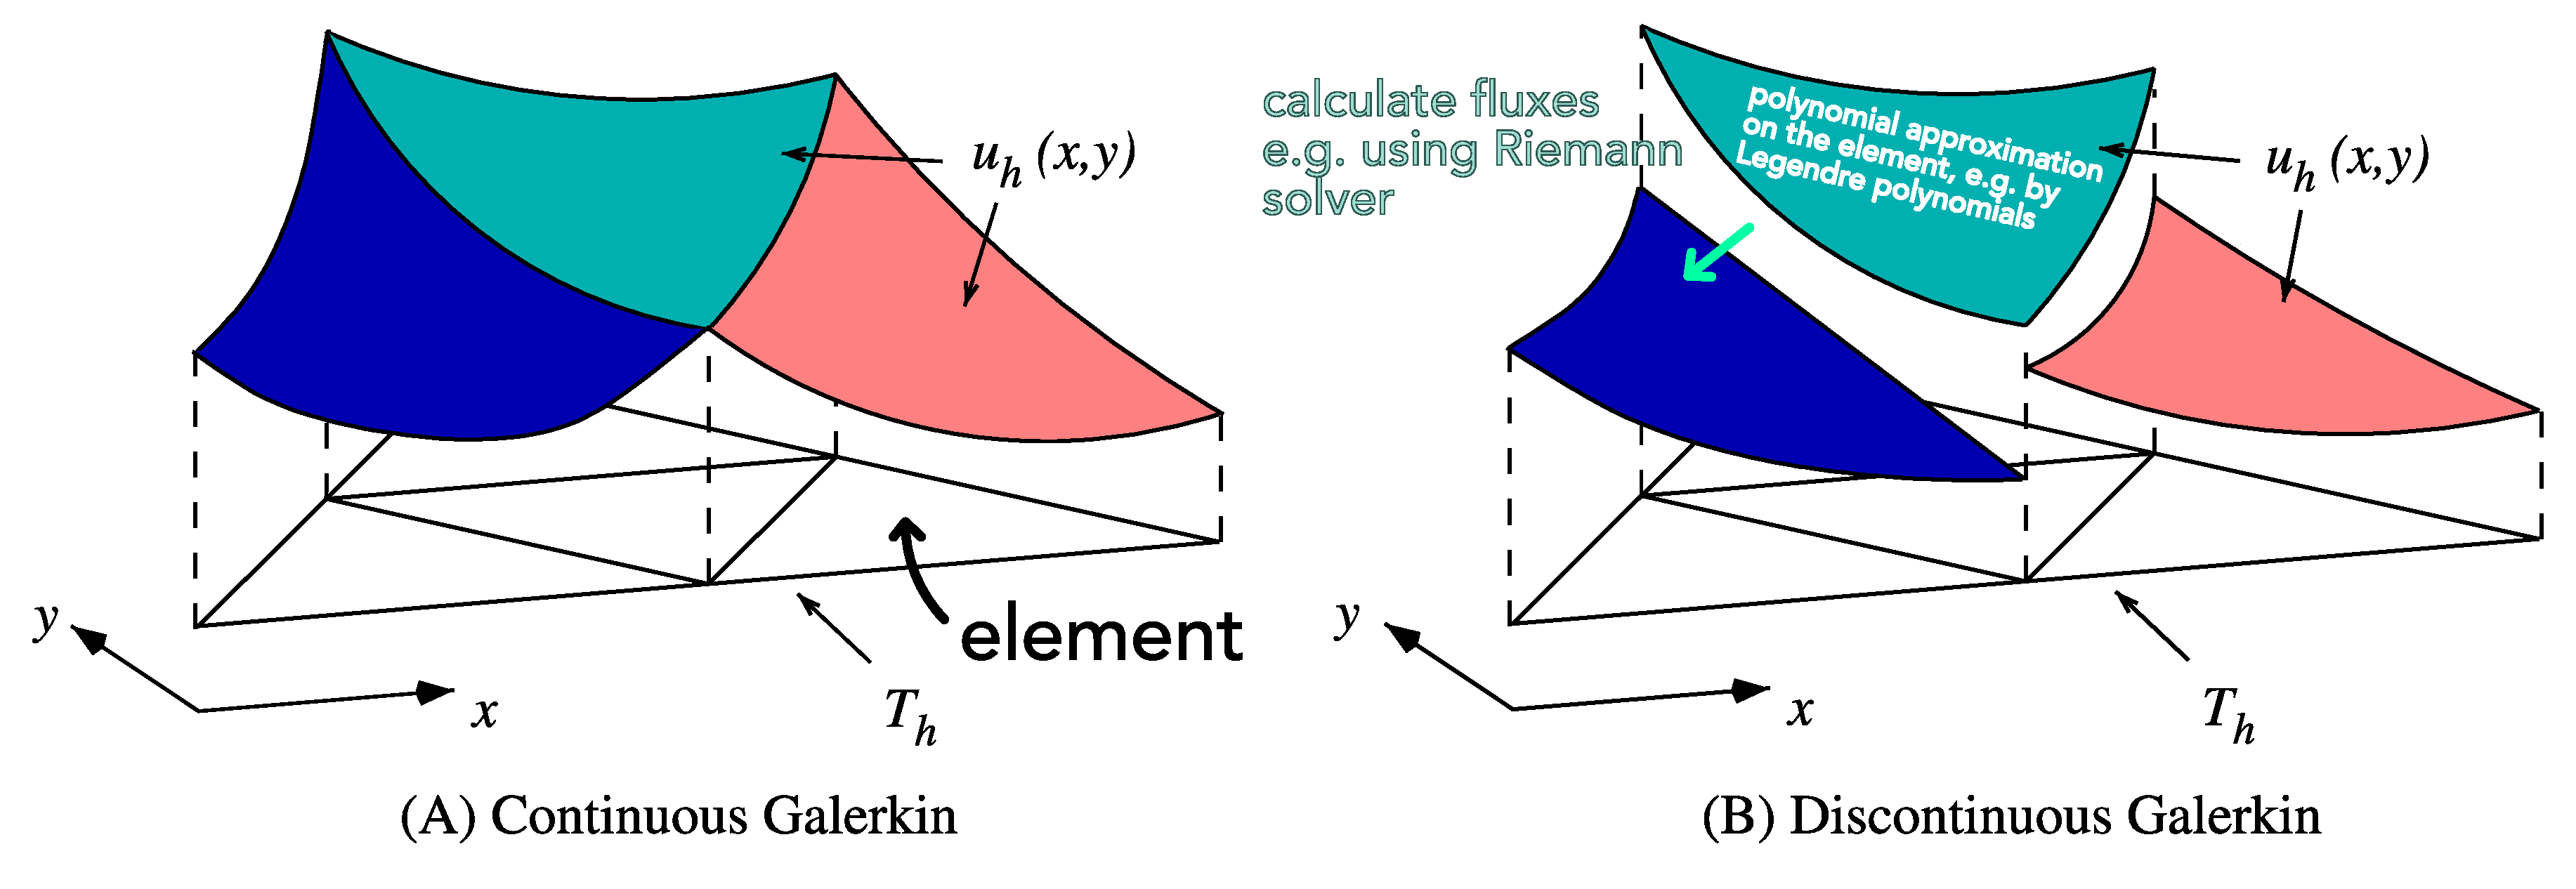
\includegraphics[width=0.8\textwidth]{figures/DG.pdf}
    \caption{Continuous and discontinuous Galerkin}
    \label{fig:continuous_discontinuous_galerkin}
\end{figure}

\subsubsection{Problem we want to tackle | Euler equations}
Consider the 3D formulation of the Euler equations we know from dimensional splitting
\begin{equation}
    \begin{gathered}
        \partial_t \vec{u}(\vec{x}) + \sum_{\alpha = 1}^{3} \partial_{x_\alpha} \vec{f}_\alpha (\vec{u}) = 0, \quad \text{state vector } \vec{u} = \left(\begin{array}{c} \rho \\ \rho \vec{v} \\ \rho e \end{array} \right) \\
        \text{specific energy } e = \rho e_{th} + \frac{1}{2} \rho \vec{v}^2 \text{ with specific internal energy } e_{th}
    \end{gathered}
\end{equation}
with flux vectors
\begin{equation}
    \begin{gathered}
        \vec{f}_1=\left(\begin{array}{c}
            \rho v_1 \\
            \rho v_1^2+P \\
            \rho v_1 v_2 \\
            \rho v_1 v_3 \\
            v_1(\rho e+P)
            \end{array}\right), \quad \vec{f}_2=\left(\begin{array}{c}
            \rho v_2 \\
            p v_1 v_2 \\
            \rho v_2^2+P \\
            \rho v_2 v_3 \\
            v_2(\rho e+P)
            \end{array}\right), \quad \vec{f}_2=\left(\begin{array}{c}
            \rho v_3 \\
            p v_1 v_3 \\
            \rho v_2 v_3 \\
            \rho v_3^2+P \\
            v_3(\rho e+P)
            \end{array}\right) \\
            \text{ideal gas closure } P = \rho e_{th} (\gamma - 1)
    \end{gathered}
\end{equation}

\bluebox{\textbf{Aim: } From a given initial state $\vec{u}(\vec{x}, t = 0) = u(\vec{x},0)$ we want to find the subsequent evolution of the fluid.}

\subsubsection{Steps in formulating the Dicontinuous Galerkin (DG) scheme}
\begin{enumerate}
    \item Subdivide the space into elements aka cells
    \item Represent the fluid state on a cell using a polynomial basis (e.g. Legendre polynomials) with weights evolving in time; \textit{nodal} vs \textit{modal}
    \item Find a general formula for the weights in the \textit{modal} variant
    \item Find the initial weights from specific \textit{nodal} starting values in the \textit{modal} scheme
    \item Find an evolution equation for the weights
\end{enumerate}

\subsubsection{Subdivision and Representation | modal vs nodal}
\yellowbox{The fluid state is represented as a polynomial approximation (for the respective fluid variables) on the element (non overlapping elements with discontinuities in-between) - but how?}
A typical DG cell is illustrated in figure \ref{fig:dg_cell}.

\begin{figure}[!htb]
    \centering
    \includesvg[width=0.8\textwidth]{figures/DGcell.svg}
    \caption{Typical DG cell}
    \label{fig:dg_cell}
\end{figure}

There are two possible representations of the solution
\begin{itemize}
    \item \textbf{nodal}: We store and operate on fluid state vectors at chosen positions within the cell. In the Legrange interpolation with Lagrange polynomials of degree $k$, so $l_j(x) = \prod_{\begin{array}{c} 0 \leq m \leq k \\ m \neq j \end{array}} \frac{x - x_m}{x_j - x_m}$, for one fluid variable the node values are also the expansion coefficients, $u = \sum_{j=0}^{N(k)} u_j l_j(x)$. The positions of the nodes in the cell are chosen smartly regarding quadrature (integration) rules.
    \item \textbf{modal}: We store and operate on weights of usually orthogonal polynomials (usually Legendre). Integrals are still evaluated using quadrature rules. Initial weights have to be calculated based on nodal values.
\end{itemize}

We opt for \textbf{modal}.

The solution in the interior of \textcolor{yellow1}{cell $K$} is given by a linear combination of $N(k)$ orthogonal 
and normalized basis functions $\phi_l^{(K)}$ (maximum degree of the basis functions is $\mathcolor{green1}{k}$).

\begin{equation}
    \vec{u}^{\mathcolor{yellow1}{(K)}}(\vec{x}, t)=\sum_{l=1}^{N(\mathcolor{green1}{k})} \vec{\omega}_l^{\mathcolor{yellow1}{(K)}}(t) \phi_l^{\mathcolor{yellow1}{(K)}}(\vec{x})
\end{equation}

where
\begin{itemize}
    \item the space-time dependence of the fluid state was split into time dependent weights and space dependent basis functions
    \item the cell's state is completely given by the $N(k)$ weights
\end{itemize}

\subsubsubsection{Example for an orthogonal polynomial basis: Legendre polynomials}
We can combine Legendre polynomials to 3D base functions with degree up to $k$, leading to a $p=k+1$th order
scheme in space, in the following manner
\begin{equation}
    \begin{gathered}
        \left\{\phi_l(\vec{\xi})\right\}_{l=1}^{N(k)}=\left\{\tilde{P}_u\left(\xi_1\right) \tilde{P}_v\left(\xi_2\right) \tilde{P}_w\left(\xi_3\right) \mid u, v, w \in \mathbb{N}_0 \wedge u+v+w \leq k\right\} \\
        \text { scaled Legendre polynomials } \tilde{P}_n(\xi)=\sqrt{2 n+1} P_n(\xi) \\
        \text { "special orthog. " } \int_{-1}^1 P_i(\xi) P_j(\xi) d \xi= \begin{cases}0 & \text { if } i \neq j \\ 2 & \text { if } i=j\end{cases}
    \end{gathered}
\end{equation}
For a polynomial basis with maximum degree $k$ we have
\begin{equation}
    N(k)=\sum_{u=0}^k \sum_{v=0}^{k-u} \sum_{w=0}^{k-u-v} 1
\end{equation}
basis polynomials.

The first Legendre polynomials are

\begin{equation}
    P_0(\xi)=1, P_1(\xi)=\xi, P_2(\xi) = \frac{1}{2}\left(3 \xi^2-1\right)
\end{equation}

\note{The span of ${P_0(x),P_1(x),\dots,P_n(x)}$ is the same as of ${1,x,x^2,\dots,x^n}$. So
\begin{equation}
    \forall \text{polynomial } P \text{ of degree } < n: \int_{-1}^{1} P(x) P_n(x) \, d x=0
\end{equation}
}

\subsubsection{Solving for the weights}
\note{The main application of finding weights is finding the weights of the initial state. Going from weights to evaluations is easy.}
Let's say we would know $\vec{u}^{\mathcolor{yellow1}{(K)}}(\vec{x}, t)$ - then we can determine the weights
based on the orthogonality and normalization properties of the basis functions as
\begin{equation}
    \label{eq:dg_weights_integral}
    \begin{gathered}
        \vec{\omega}_j^K(t)=\frac{1}{|K|} \int_K \vec{u}^{(K)} \phi_j^{(K)} d V, \quad j=1, \ldots, N(k) \\
        \text { with } |K| \text { volume of cell } K
    \end{gathered}
\end{equation}
We hereby choose $\phi_1^{(K)} = 1$ so that $\omega_1^{(K)}$ is the cell's average of the 
state vector $\vec{u}^{(K)}$ (constant term). $\phi_j^{(K)}, j\geq 2$ are higher order basis functions,
with $w_j^{(K)}$ being the higher order moments of the state vector $\vec{u}^{(K)}$.

\yellowbox{\textbf{Scaled variable on cell:} On a cube, we can define the basis functions in terms of 
a scaled variable $\vec{\xi}$.
\begin{equation}
    \label{eq:dg_scaled_variable}
    \begin{gathered}
        \phi_l(\vec{\xi}): [-1,1]^3 \rightarrow \mathbb{R}, \quad \vec{\xi} = \frac{2}{\Delta x} \left( \vec{x} - \vec{x}^{(K)} \right) \\
        \text{cell's center } \vec{x}^{(K)}, \text{ cell's sidelength } \Delta x
    \end{gathered}
\end{equation}
}

\idea{Let us approximate this integral by a quadrature rule.}
First write the integral equation for the weights in the reference frame of a cubic cell with sidelength $2$
\begin{equation}
    \vec{\omega}_j^{(K)}(t)=\frac{1}{8} \int_{[-1,1]^3} \vec{u}^{(K)}(\vec{\xi}, t) \phi_j^{(K)}(\vec{\xi}) d^3 \vec{\xi}, \quad j=1, \ldots, N(k)
\end{equation}
We then apply Gauss-Legendre quadrature with $(k+1)^3$ quadrature points, so
\begin{equation}
    \label{eq:dg_weights}
    \begin{gathered}
        \vec{\omega}_j^{(K)}(t) \approx \frac{1}{8} \sum_{q=1}^{(k+1)^3} \vec{u}^{(K)}\left(\vec{\xi}_q^{3 D}, t\right) \phi_j^{(K)}\left(\xi_q^{3 D}\right) w_q^{3 D}, \quad j=1, \ldots, N(k) \\
        \text{positions of quadrature nodes in cell's reference frame } \vec{\xi}_q^{3 D}, \text{ quadrature weights } w_q^{3 D}
    \end{gathered}
\end{equation}
\subsubsubsection{What even is Gauss-Legendre quadrature?\skipthis}
It is intuitive that an integral can be approximated by the mean of evaluation points.
However, it turns out, that one can exactly integrate polynomials of degree $2n-1$ with $n$ smart
evaluation points and weights. One such method is called Gauss-Legendre quadrature.

\textbf{Claim: } The approximation
\begin{equation}
    \begin{gathered}
        \int_{-1}^1 f(\xi) d \xi \approx \sum_{q=1}^n f\left(\xi_q^{1 D}\right) w_q^{1 D} \\
        \text{roots } \xi_q^{1 D} \text{ of } P_n(\xi), \text{ weights } w_q^{1 D}=\frac{2}{\left(1-\left( \xi_{q}^{1 D} \right)^2\right)\left(P_{n}^{\prime}\left(\xi_{q}^{1 D}\right)\right)^{2}}
    \end{gathered}
\end{equation}
for $f: [-1,1] \rightarrow \mathbb{R}$ is exact for polynomials of degree $2n-1$.

\textbf{Proof: } Let $f = P(x)$ have degree $\leq 2n-1$. Then we can write
$P(x) = Q(x) P_{n+1}(x) + R(x)$ with $Q(x), R(x)$ polynomials of degree $\leq n$ ($P_{n+1}(x)$ is the $(n+1)$-th Legendre polynomial).
Then 
\begin{equation}
    \begin{aligned}
        \int_{-1}^{1} P(x) d x &=\underbrace{\int_{-1}^{1} Q(x) P_{n+1}(x) d x}_{=0\text{ as } Q \text{ can be written in base } \{P_0,\dots,P_n\} \perp P_{n+1}}+\int_{-1}^{1} R(x) d x \\
        &=\int_{-1}^{1} R d x \\
        &=\underbrace{\sum_{q=1}^{n} R\left(\xi_{q}^{1 D}\right) w_{q}^{1 D}}_{\text{exact as } R \text{ is a polynomial of degree } \leq n} \\
        &=\sum_{q=1}^{n} \left( R\left(\xi_{q}^{1 D}\right) + \underbrace{P_{n+1}(\xi_{q}^{1 D}) \cdot Q(\xi_{q}^{1 D})}_{=0, \text{as } \xi_{q}^{1 D} \text{ roots of } P_{n+1}} \right)w_{q}^{1 D} \\
        &= \sum_{q=1}^{n} P(\xi_{q}^{1 D}) w_{q}^{1 D}
    \end{aligned}
\end{equation}

\textbf{Formulation in higher dimensions: } We generalize to $f: [-1,1]^2 \rightarrow \mathbb{R}$ by
\begin{equation}
    \int_{-1}^1 \int_{-1}^1 f\left(\xi_1, \xi_2\right) d \xi_1 d \xi_2 \approx \sum_{q=1}^n \sum_{r=1}^n f\left(\xi_q^{1 D}, \xi_r^{1 D}\right) w_q^{1 D} w_r^{1 D}=\sum_{q=1}^{n^2} f\left(\vec{\xi}_q^{2 D}\right) w_q^{2 D}
\end{equation}

\subsubsection{Finding initial weights - just apply the determination of weights to the initial state}
The initial state $\vec{u}(\vec{x}, t=0)$ is best represented by weights $\vec{\omega}_j^{(K)}(t=0)$, such that

\begin{equation}
    w_{l,i}^{(K)}(t=0)= \argmin_{\vec{\omega}_{j,i}^{(K)}(t=0)} \int_{K} \left( u_i^{(K)}(\vec{x}, t=0) - u_i(\vec{x}, t=0) \right)^2 d^3 \vec{x}, \quad i \text{ over state vector components}
\end{equation}

which just leads us to the previous projection (eq. \ref{eq:dg_weights_integral}) and solution in eq. \ref{eq:dg_weights} at $t=0$, where
our initial state must be known on the quadrature nodes.

\subsubsection{Evolution equation for the weights}

We derive a DG scheme on cell $K$.

\textcolor{blue1}{Weak form of the Euler equations}: A weak formulation of the Euler equations
for the polynomial approximation $\vec{u}^{(K)}$ on cell $K$ is found by multiplying the Euler equations
with the basis function $\phi_j^{(K)}$ and integrating over the cell $K$.
\begin{equation}
    \int_K\left[\partial_t \vec{u}^{(K)}+\sum_{\alpha=1}^3 \partial_{x_\alpha} f_\alpha\right] \phi_j^{(K)} d V=0
\end{equation}
Integrating by parts and applying Gauss theorem, we get
\begin{mdframed}
\begin{equation}
    \begin{gathered}
        \frac{d}{d t} \underbrace{\int_K \vec{u}^{(K)} \phi_j^K d V}_{\vec{w}_j^{(K)} \cdot |K|} + \sum_{\alpha=1}^3 \explain{\int_{\partial K} f_\alpha n_\alpha \phi_j^K d S}{evaluate using Gauss-Quad, unknown flux across discont. via Riemann solver} - \sum_{\alpha=1}^3 \explain{\int_K \vec{f}_\alpha \frac{\partial \phi_j^K}{\partial x_\alpha} d V}{evaluate via Gauss-Quad., interior flux known from state variable approx.} = 0 \\
        \text{normal vector } \vec{n} = \left( \begin{array}{c} n_1 \\ n_2 \\ n_3 \end{array} \right) \text{ on } \partial K
    \end{gathered}
\end{equation}
- we have found a system of coupled ODEs for the weights which can be solved for instance using RK schemes.
Remember to transform to the cell coordinates \\ $\left( d\xi^3 = \left( \frac{2}{\Delta x^{(K)}} \right)^2 dV \right)$
(from eq. \ref{eq:dg_scaled_variable}).
\end{mdframed}

Note on strong shocks: In case there are strong shock waves, limiting-schemes damping oscillations (e.g. by setting higher expansion
coefficients in cells adjacent to the detected discontinuity to zero) are used.

\subsubsection{Efficiency of DG and refinement schemes}
Accuracy can be increased by
\begin{itemize}
    \item \textcolor{green1}{p}-refinement: higher order scheme (polynomials up to higher order degree in the basis set)
    \item h-refinement: finer grid with smaller spacing
\end{itemize}

In both cases, the number of weights increases. For isentropic vortex flow, one finds that p-refinement is much
more efficient (better solution at less CPU time) than h-refinement.

\todo[inline]{more on nodal vs modal, more details from script}

\pagebreak